\documentclass[12pt]{article}

\usepackage{ucs}
\usepackage[utf8x]{inputenc} 		% Включаем поддержку UTF8
\usepackage[russian]{babel}  		% Включаем пакет для поддержки русского языка

\usepackage[
	left=2cm, 			% Поле левое : 200 мм
	right=2cm, 			% Поле правое : 200 мм
	top=2cm,			% Поле верхнее: 200 мм
	bottom=2cm,			% Поле нижнее : 200 мм
	bindingoffset=0cm]{geometry}

\usepackage[pdftex]{graphicx, color}
\usepackage{color}
\usepackage{tikz}
\usepackage{url}			% использование URL в библиографии
\usepackage{listings}			% использование листингов кода
\usepackage[nooneline]{caption} 
\captionsetup[table]{justification=raggedleft} 
\captionsetup[figure]{justification=centering,labelsep=endash}
\usepackage{array}

\usepackage{caption}
\usepackage{graphicx}
\usepackage{subcaption}
\usepackage{cases}

\renewcommand{\baselinestretch}{1.5}

% вставка листингов с кодом
\lstset{inputencoding=utf8x,
		extendedchars=false,
		keepspaces=true,
		language=c}

\renewcommand{\lstlistingname}{Листинг}

%\usepackage{amsmath}
%\usepackage{mathtools}
\setcounter{tocdepth}{4} 	% chapter, section, subsection, subsubsection и paragraph
\setcounter{secnumdepth}{4}

\parindent=1,25cm				% красная строка = 1 см
\usepackage{enumitem}
\setlist[enumerate,1]{leftmargin=2.25cm}
\setlist[itemize]{leftmargin=2.25cm}
\graphicspath{{pics/}}
\lstset{inputpath="./snippets/"}
\DeclareGraphicsExtensions{{.jpg}}

\begin{document}
	\part*{\centering Введение}
	\addcontentsline{toc}{part}{Введение} % добавление раздела в оглавление
	\hspace{\parindent} Проект {\it GW-Basic} представляет собой среду разработки приложений, а также диалект языка программирования {\it Basic}. Среда разработки предоставляет пользователю возможности для написания программ на одноименном языке, вычисление вычисление выражений путем интерпретации запроса после ввода, а также визуализацию графики. \\
	\indent В данной работе рассматривается реализация среды исполнения {\it GW-Basic} с использованием средств генерации анализаторов одноименного языка (инструменты {\it flex}, {\it bison}), а также создание графической оболочки для взаимодествия со средой средствами {\it OpenGL} и инструментарием {\it glut}. 
	\newpage
	\section{Обзор используемых технологий}	
		\subsection{Среда разработки GW-Basic}
			% Здесь нужно рассказать в общем про среду разработки, дату появления.
			\hspace{\parindent} Среда разработки Microsoft GW-Basic, а также одноименный язык программирования представляют собой платформу для написания программ в императивной нотации. 
			% Что из себя представляет
			Управление средой осуществляется с помощью командной строки, в которую попадает пользователь после запуска.
			\subsubsection{Cинтаксические конструкции}
			\label{subsec:basicKeywords}
			% Commands, Statements, Variables, Expressions, ...
			% 2.4 Ingleese	
			\hspace{\parindent} Программа на GW-Basic может включать в себя следующие синтаксические конструкции \cite{basicManual}:
			\begin{itemize}
				\item {\bf Ключевые слова} (англ. {\it Keywords}) -- представляют собой зарезервированные слова среды исполнения GW-Basic, и являются частью операторов или команд. 				
				\item {\bf Команды} (англ. { \it Commands}) -- это исполняемые инструкции. Выполнение команд осуществляется сразу после ввода.
				\item {\bf Операторы} (англ. {\it Statements}) -- являются исполняемыми инструкциями программы на GW-Basic. Представляют собой группу ключевых слов, используемых как строки программы среды GW-Basic.
				\item {\bf Функции} (англ. {\it Funtions}) -- по типу возвращаемых значений могут быть: строковыми, численными. 
				\item {\bf Переменные} (англ. {\it Variables}) -- определенная строка, за которой установлено определенное значение. Переменные могут быть объявлены/изменены как пользователем, так и контекстом программы.
			\end{itemize}

			% Про то, что ключевые слова с большой буквы
			\indent Ключевые слова (имена команд, операторов) представляют собой последовательность заглавных латинских букв. Примерами ключевых слов в GW-Basic являются слова: {\tt PRINT}, {\tt RETURN}, {\tt GOTO}. Ключевые слова не могут быть использованы в качестве имен переменных, иначе это бы привело к конфликту с такими синтаксическими конструкциями, как {\it Команды} и {\it Операторы}. \\
			% Подробнее про функции и переменные, про типы значений (строковые и численные) cимвол обязательно должне вначале идти.
			\indent Имена функций и переменных могут включать в себя: буквы латинского алфавита, цифры, символ {\tt '.'}. Также, имена могут начинаться только с латиской буквы.
			
			\indent Список всех синтаксических конструкций представлен в \cite[стр.~117]{basicManual}.
			\subsubsection{Режимы интерпретации запросов}
			\label{subsec:interpTypes}
			% Direct, Indirect
			% 2.5 Line Format
			\hspace{\parindent} Интерпретация пользовательских запросов в среде GW-Basic может проходить в следующих режимах:
			\begin{enumerate}
				\item {\bf Прямой} (англ. {\it Direct}) 
				\item {\bf Непрямой} (англ. {\it Indirect}) 
			\end{enumerate}
			
			\indent В {\it прямом режиме}, введенные операторы и команды исполняются сразу после окончания ввода. Этот режим используется преимущественно в целях отладки программы, либо для вычисления выражений, для которых нет необходимости писать программу. \\
			\indent {\it Непрямой режим} используется для создания/редактирования строк программы. Каждая строка программы на GW-Basic имеет следующий формат:
			\begin{center}
				\tt nnnnn statement[statements]
			\end{center}

			\indent	Где {\tt nnnnn} -- номер строки, a {\tt statement} -- оператор GW-Basic. В зависимости от логики программы, строка может содержать более одного оператора ({\tt [statements]}). В этом случае, операторы должны быть разделены символом двоеточия {\tt ':'}. Для запуска программы, используется команда {\tt RUN}.\\
			\indent Полное руководство по редактированию программы в среде GW-Basic представлено в \cite[стр.~18]{basicManual}.

			\subsubsection{Графический режим}
			\label{subsec:graphixMode}
			% SCREEN 12
			\hspace{\parindent} Согласно \cite[стр.~142]{basicManual}, среда выполнения GW-Basic имеет несколько режимов визуализации информации на экране. Использование команды {\tt SCREEN} позволяет изменять режим вывода среды с целью включения/отключения/изменения графического режима. По умолчанию, т.е. при запуске среды без использования этой команды, среда работает в {\it текстовом режиме}, что означает, что выполнение любого оператора, связанного с графикой, будет проигнорировано. \\
			\indent При активации {\it графического режима}, пользователю становится доступно использование графических операторов. Среда GW-Basic предлагает визуализацию следующих примитивов: {\tt CIRCLE}, {\tt LINE}, {\tt POINT}, и т.д. Полный список операторов представлен в \cite[стр.~117]{basicManual}. 
			% страница 142 (Screen) 137 (Circle) 155 (Line)

		\subsection{Flex и Bison -- инструменты разработки анализаторов}
		% описать про flex
		\hspace{\parindent} В процессе развития теории построения компиляторов, сформировалось множество подходов к обработке и анализу программ различных языков программирования. Наиболее популярный из них заключается в разбиении задачи разбора на два этапа \cite[стр.~21]{flexManual}:
		\begin{enumerate}
			\item {\bf Лексический анализ программы} (англ. {\it Scanning}) -- сканирование текста программы с целью выделения {\it токенов} (англ. {\it Tokens}), а также значений, которые стоят за этими токенами.
			\item {\bf Синтаксический разбор} (англ. {\it Parsing}) -- установление связей между токенами, называемых {\it правилами грамматики}. 
		\end{enumerate}
		
		\indent Для выполнения лексического разбора, наиболее популярным генератором анализатора является {\it flex}. В основе выделения токенов лежит использование регулярных выражений. Что касается генерации синтаксического анализатора, то для этих целей широко применяется {\it bison}. Для описания связей между токенами, {\it bison} использует нотацию правил грамматики в форме Бэкус-Наура.	
		\subsection{Glut -- инструментарий для работы с OpenGL}
		% описать про glut
		\hspace{\parindent} {\it Glut} представляет собой оконно-независимый инструмент для написания программ на {\it OpenGL}. Инструментарий поддерживает {\it функции обратного вызова} (англ. {\it Callback functions}) для большинства событий \cite{glutCallbacks}. В частности, наиболее используемые функции обратного вызова:
		\begin{itemize}
			\item {\bf glutDisplayFunc} -- вызывается при отрисовке сцены.
			\item {\bf glutReshapeFunc} -- используется для обработки события изменения размера окна.
			\item {\bf glutKeyboardFunc} -- вызывается в случае возникновения нажатия клавиши.
		\end{itemize}
		
	\newpage
	\section{Разработка среды GW-Basic}
		\subsection{Анализаторы языка GW-Basic}
			% какие анализаторы будут разработаны?
			\subsubsection{Лексический анализатор}
			\label{subsec:lexAnalyzer}
				% элементы лексического анализатора (название команд, операторов, ф-ций, ...) (согласно тому, какие могут быть конструкции языка)
				\hspace{\parindent} Рассмотрим основные конструкции, которые необходимо выделить в лексемы:
				\begin{enumerate}
					\item Ключевые слова
					\item Имена функции и переменных.
					\item Константные значения: численные и строковые.
					\item Символы (арифметических операций, операций сравнения, операторы логики).
				\end{enumerate}
				
				\indent Создание переменных или функций, названия которых совпадает с названием ключевых слов недопустимо \cite{basicManual}. Это означает, что приоритет за определением ключевых слов, и что разбор имен функций и переменных должен идти после разбора ключевых слов. Что касается константных значений и символов, то распознавать эти синтаксические конструкции можно на любом этапе.
			\subsubsection{Синтаксический анализатор}
			\label{subsec:syntaxAnalyzer}
				% Основываясь на 1.1 (Ingleese GWBasic), описать что есть Direct/Indirect Mode
				\hspace{\parindent} Целью использования синтаксического анализатора является построение {\it дерева синтаксического разбора} (англ. {\it AST-Tree}). Поскольку среда разработки GW-Basic представляет собой командную строку, то синтаксический разбор должен производится для каждого пользоватлеского запроса. Учитывая режимы интерпретации команд (см. п.~\ref{subsec:interpTypes}), сокращенная форма грамматики в нотации Бэкус-Науровой формы, выглядит следующим образом (см. листинг~\ref{code:syntaxGrammar}):
				\lstinputlisting[frame=single, basicstyle=\footnotesize, caption={Грамматика синтаксического анализатора языка GW-Basic.}, label={code:syntaxGrammar}]{syntax_grammar.txt}
				
				\indent Грамматика для переменных языка GW-Basic представлена в листинге \ref{code:varGrammar}. Под терминалом {\tt DECLARATION} понимается объявление имени функции или переменной. Символы, следующие за этим терминалом, указывают на тип значения переменной.
				% Конструкции языка (Операторы, выражения, команды). а затем, из чего они состоят
				\lstinputlisting[frame=single, basicstyle=\footnotesize, caption={Грамматика для переменных языка GW-Basic.}, label={code:varGrammar}]{var_grammar.txt}
				
				% Выражения языка GW-Basic
				\indent Для вычисления значений, как с целью вывода результата, так и для определения присваемого значения переменной, необходимо определить грамматику {\it выражений} (англ. {\it Expressions}) (сокращенный вариант, см. листинг \ref{code:exprGrammar}). Поскольку значения переменных могут быть строкового или численного типа, то и выражения могут быть тоже двух типов. 
				\lstinputlisting[frame=single, basicstyle=\footnotesize, caption={Грамматика для выражений языка GW-Basic.}, label={code:exprGrammar}]{expr_grammar.txt}
				

				\indent Для строк, среда GW-Basic предоставляет единственную бинарную операцию -- конкатенацию. В свою очередь, численные выражения разбиваются на четыре класса (см.~\cite[стр.~46]{basicManual}):
				\begin{itemize}
					\item {\bf Арифметический оператор} -- выполнение бинарных операций {\tt '+', '-', '\^\ ', '/'}.
					\item {\bf Логический оператор} -- выполнение булевских операций {\tt NOT, AND, OR, XOR}, и т.д. 
					\item {\bf Функциональный оператор} -- математические/строковые функции.
					\item {\bf Оператор отношения} -- выполнение бинарных операций {\tt '>', '<', '=', '<=', '>='}, и т.д.
				\end{itemize}
				% Написать только до момента появляения команд,операторов,фунций
		\subsection{Архитектура системы исполнения}
			\label{subsec:runtimeArch}
			% схема, поэтапная, расширяющаяся
			\hspace{\parindent} Архтектура системы исполнения представлена на рис. \ref{fig:runtimeArch}. Компоненты системы исполнения представлены блоками, а зависимость между блоками обозначена стрелочками. 	
			\begin{figure}[h]
				\center{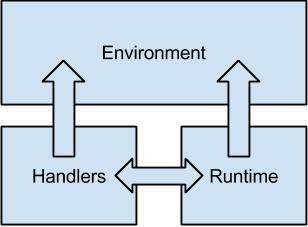
\includegraphics[scale=0.6]{runtime_arch.jpg}}
				\caption{Архитектура системы исполнения}
				\label{fig:runtimeArch}
			\end{figure}
			
			\indent Рассмотрим компоненты системы исполнения подробнее. 
			
			\subsubsection{Окружение среды}
			\label{subsec:environment}
			\hspace{\parindent} {\it Окружение} (англ. {\it Environment}) включает в себя структуру, которая хранит текущее состояние интерпретатора, а также набор функций для изменения содержимого структуры. Чтобы описать текущее состояние, структура должна содержать следующую информацию:
			\begin{itemize}
				\item Режим работы интерпретатора.
				\item Привязку к системе вывода/вывода.
				\item Контекст выполнения.
			\end{itemize}
			
			\indent Интерпретатор среды должен поддерживать следующие режимы работы (согласно п. \ref{subsec:interpTypes}):
			\begin{enumerate}
				\item Интерпретацию команд.
				\item Выполнение программы на GW-Basic.
			\end{enumerate}
			% Парсер, написать со ссылкой на предыдущий раздел
			\subsubsection{Обработка пользовательских запросов}
			% обработчики, и то что для каждой вершины AST дерева, есть соответсвующий обработчик в системе выполнения. 
			\hspace{\parindent} Компонент {\it обработки вершин дерева синтаксического разбора} (англ. {\it AST-Node Handler}) (см. рис.~\ref{fig:runtimeArch}, {\it Handlers}), представляет собой набор функций для обработки вершин дерева. Под процессом обработки вершины понимается внесение изменений в {\it контекст исполнения} (см. п.~\ref{subsec:environment}). Так, для каждого типа вершины дерева, существует в точности единственная функция обработки. \\
			\indent Каждая функция обработки, должна иметь следующие входные параметры:
			\begin{itemize}
				\item Окружение системы исполнения.
				\item Вершину дерева синтаксического разбора, тип которой соответствует типу функции.
			\end{itemize}
			
			% связь обработчика вершины с обработкой дочерних узловых вершин	
			\indent Поскольку вершина является элементом дерева, то обработка дочерних вершин осуществляется методом рекурсивного спуска.

			\subsubsection{Выполнение команд и программы}
			% Обработка команд (сразу после ввода, выполнение всей программы)
			\hspace{\parindent} За выполнение пользовательских команд отвечает {\it система времени выполнения} (англ. {\it Runtime}) (см. рис.~\ref{fig:runtimeArch}). Согласно п.~\ref{subsec:interpTypes}, синтаксис записи команд влияет на режим выполнения этих команд средой. В тоже время, режимы выполнения учитываются грамматикой синтаксического анализатора (см. п.~\ref{subsec:syntaxAnalyzer}), поэтому реализация {\it прямого} и {\it непрямого} режимов полностью ложится на обработчики соответствующих вершин дерева синтаксического разбора. \\   
			\indent Таким образом, процесс выполнения пользовательского запроса состоит из следующих этапов:
			\begin{enumerate}
				\item Чтение пользовательского запроса.
				\item Применение анализаторов (п. \ref{subsec:lexAnalyzer}, \ref{subsec:syntaxAnalyzer}) c целью построения дерева синтаксического разбора.
				\item Обработка корневого узла дерева с помощью соответствующего обработчика.
			\end{enumerate}

			\indent Рассмотрим особенности выполнения программы на GW-Basic. В процессе выполнения программы, может возникнуть необходимость ее временной остановки. Пример такой ситуации -- ожидание ввода значения перемнной-аргумента оператора {\tt INPUT}. Таким образом, процесс выполнения программы на GW-Basic состоит из следующих этапов:
			\begin{enumerate}
				\item Чтение пользовательской команды {\tt RUN}.
				\item В обработчике команды, осуществляется смена режима окружения на {\it выполнение программы}.
				\item Выполнение программы, путем вызовов обработчиков инструкций кода.
				\item Обработчик инструкции {\tt INPUT} останавливает выполнение программы, поскольку требуется входные данные соответствующей инструкции. После ввода данных, необходимо продолжить выполнение программы (этап 3).
				\item Завершение выполнения, смена режима окружения на {\it интерпретации команд}.
			\end{enumerate}
			% про то, что в в каждой строке храница вершина AST -- это нужно написать в реализации.
			\subsection{Среда разработки в графическом режиме}
			\label{subsec:ideArch}
			% наличие холста
			\hspace{\parindent} Графический режим среды исполнения позволяет интерпретировать графические команды GW-Basic (см. п.~\ref{subsec:graphixMode}). В отличие от текстового режима, в графическом режиме требуется введение {\it холста} (англ. {\it Canvas}) -- область, на которой отображается результат выполнения графической команды GW-Basic. \\ 
			\indent В тоже время, возможность ввода текста должна быть сохранена, поэтому необходимо ввести {\it матрицу текста}, которая будет отображать следующую информацию:
			\begin{enumerate}
				\item Пользовательский запрос в процессе ввода.
				\item Результат выполнения неграфических команд.
			\end{enumerate}

			% выводом данных
			\indent В отличие от текстовой информации, графическая отображаеся только после выполнения соответствующей инструкции. Для исключения возможности перекрытия текста графикой, визуализацию кадра необходимо выполнять в следующей последовательности:
			\begin{enumerate}
				\item Отображение холста.
				\item Отображения текущей матрицы текста.
			\end{enumerate}
			
	\newpage
	\section{Реализация среды GW-Basic}
		% Реализация среды на C (К вопросу о языке разработки), 
		\hspace{\parindent} Реализация среды разработки GW-Basic осуществлялась на языке C. В результате, пользователю доступны исполняемые файлы со следующими режимами работы консоли:
		\begin{enumerate}
			\item Консоль текстового режима (исполнение только неграфических команд).
			\item Консоль графического режима (исполнение текстовых и графических команд).
		\end{enumerate}
		
		%\indent Реализацией не предусматривается возможность перехода среды из текстового режима в графический. Но в тоже время, графический режим включает в себя полную поддержку текстового.
		\subsection{Лексический и синтаксический анализаторы}
			% Использование инструментов Flex и Bison
			\hspace{\parindent}Генерация лексического анализатора осуществлялась с помощью инструмента {\it flex}.
			% Ссылки на соответствующие пункты разработки + в приложении разместить грамматику
			% Написать про то, что для каждого нетерминала была создана своя структура
			\indent За генерацию синтаксического анализатора отвечает инструмент {\it bison}. Краткое описание грамматики синтаксического разбора представлено в п. \ref{subsec:syntaxAnalyzer}. \\
			\indent Посколько целью выполнения этих разборов является построение дерева синтаксического разбора, то необходимо ввести {\it структуры языка C}, объекты которых будут являться узлами этого дерева в памяти программы. Данная реализация включает {\it уникальную структуру} для каждого нетерминала грамматики (см. листинг~\ref{code:astStructsExample}):
			\lstinputlisting[numbers=left, frame=single, basicstyle=\footnotesize, caption={Пример объявления структур для вершин AST-дерева}, label={code:astStructsExample}]{ast_node_example.txt}
			
			\indent Исходя из такого подхода описания структур для каждого нетерминала грамматики (листинг \ref{code:astStructsExample}), получается что деререво синтаксического разбора полностью укладывается в корневой терминал {\tt Interpreter} (см. листинг~\ref{code:syntaxGrammar}). Если дочерний узел дерева (нетерминал) не может быть определен однозначно, то для этих целей вводится поле поле {\tt type} (например, строка 2, листинг \ref{code:astStructsExample}). 
		\subsection{Система времени выполнения}
			% Описание этих компонентов со ссылкой на реализацию на C.
			\hspace{\parindent} Одним из компонентом системы исполнения является {\it окружение}. Эта структура содержит информацию о введенных пользоватем данных, и контексте выполнения. Объявление структуры представленo в листинге \ref{code:envStruct}:
			\lstinputlisting[numbers=left, frame=single, basicstyle=\footnotesize, caption={Объявление структуры Environment, а также вложенных структур}, label={code:envStruct}]{env_struct.txt}
			
			\indent Для описания текущего режима времени исполнения используется поле {\it runtime\_type} (строка 2, листинг \ref{code:envStruct}), которое может принимать два значения (согласно п. \ref{subsec:environment}). Введенные пользователем данные хранятся в структуре {\tt GWBE\_Input} (см. листинг~\ref{code:envStruct}). \\
			\indent Рассмотрим подробнее структуры, которые требуются для описания {\it контекста выполнения}. Согласно листингу \ref{code:envStruct}, структура {\tt GWBE\_Context} включает в себя:
			\begin{enumerate}
				\item Текущую программу на GW-Basic.
				\item Переменные (среды GW-Basic, пользовательские).
				\item Стек возврата.
			\end{enumerate}
		 	
			% Про стороки программы
			\indent Поскольку любое взаимодействие со средой осуществляется с помощью пользовательских запросов, то и создание программы на GW-Basic происходит тоже с помощью запросов. За счет того, что любой запрос пользователя проходит этап обработки, вместе с текстом строк программы дополнительно хранятся вершины дерева синтаксического разбора (см. листинг~\ref{code:envProgram}). Такое решение позволяет не вызывать анализатор каждый раз при выполнении соответствующей инструкции, а сделать это один раз -- только при добавлении/замене инструкции.
			\lstinputlisting[frame=single, basicstyle=\footnotesize, caption={Представление строк программы GW-Basic}, label={code:envProgram}]{env_program.txt}
			
			% Про обработчики, со вставкой кода
			\indent Что касается реализации такого компонента системы как {\it обработчиков вершин дерева синтаксического разбора}, то сигнатуры функций выглядят следующим образом (см. листинг~\ref{code:handlers}):
			\lstinputlisting[frame=single, basicstyle=\footnotesize, caption={Пример сигнатуры обработчика вершины Interpreter}, label={code:handlers}]{handlers.txt}
			
			% про выполнение
			\indent Для определения возникновения ошибки в процессе выполнения команд, в обработчиках предусмотрена структура {\tt GWBR\_Result}, которая содержит результат выполнения обработки. Таким образом, путем вставки проверок в каждый обработчик, можно получать стек вызовов в случае возникновения ошибки в процессе обработки вершины дерева. 
		\subsection{Консоль графического режима}
			% представлением терминала
			\hspace{\parindent} В основе реализации графического режима лежит использование инструментария {\it Glut}, и библиотеки {\it OpenGL}. Согласно п. \ref{subsec:ideArch}, графический режим подразумевает отображение следующих объектов:
			\begin{enumerate}
				\item Отображение холста.
				\item Отображение текущей матрицы текста.
			\end{enumerate}
			
			% Как реализован Холст
			\indent Под холстом в данной реализации понимается матрица пикселей, на которую производится растеризация графических примитивов. Растеризация производится после выполнения очередной графической команды. Поскольку добавлять новые примитивы можно только в процессе построения кадра (т.е. в функции обратного вызова glutDisplayFunc), то отображение холста состоит из следующих этапов:
			\begin{enumerate}
				\item Загрузка холста в буфер кадра ({\tt glWritePixels} \cite{glManual}).
				\item Визуализация примитива.
				\item Чтение холста из буфера кадра ({\tt glReadPixels} \cite{glManual}).
			\end{enumerate} 

			% Как реализована матрица текста + Callback для обработки нажатий
			\indent Обновление информации в матрице текста осуществляется путем объявления {\it Glut} функции обратного вызова {\tt glutKeyboardFunc}. Обработка нажатий происходит следующим образом (см. листинг~\ref{code:handlers}):
			\begin{enumerate}
				\item При нажатии клавиши {\it backspace}, из матрицы текста {\it TextBuffer}, и из запроса пользователя удаляется последний символ (строки 2-3).
				\item При нажатии {\it enter}, производится запуск среды исолнения, а после -- очистка пользовательского запроса (строки 6-8).
				\item При нажатии любого другого символа, происходит добавление символа в матрицу текста и строку запроса (строки 11-12).
			\end{enumerate}
			\lstinputlisting[frame=single, numbers=left, basicstyle=\footnotesize, caption={Обработка нажатий клавиш}, label={code:handlers}]{keyboard_callback.txt}
				
			% Использование Glut, описать что все элементы 1.3 c точки зрения реализации на Glut
	\newpage
	\section{Тестирование}
		\hspace{\parindent} Тестирование разработанной среды GW-Basic заключается в выполнении программы, написанной на языке GW-Basic. В качестве таковой программы является игра "стрельба по мишени", исходный текст которой представлен в {\it Приложении A}.
		
		\subsection{Тестирование игры в графической консоли GW-Basic}
		\hspace{\parindent} Рассмотрим игровой процесс тестируемой игры. Игроку необходимо совершать выстрелы по мишеням, которые появляются в произвольном месте экрана. Новая мишень появляется в том случае, если игрок попал в центральное кольцо текущей. Для совершения выстрела, пользователю необходимо указать координаты стрельбы. Цель -- набрать как можно больше очков. \\ 
		\indent Демонстрация работы консоли графического режима представлена на рисунках \ref{fig:testDirect}, \ref{fig:testGame}:		
		\begin{figure}[h]
			\center{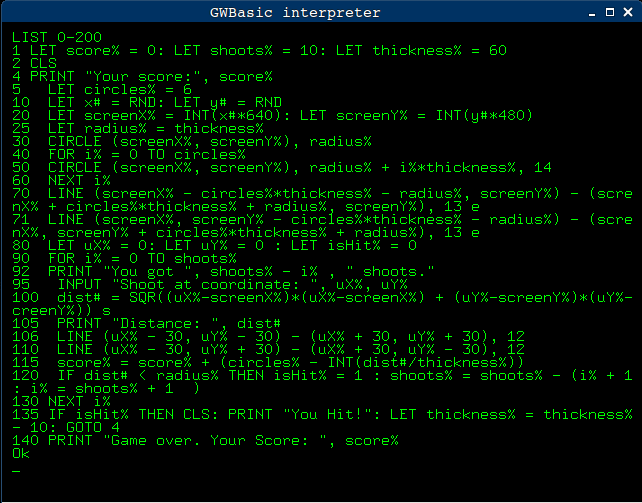
\includegraphics[scale=0.6]{gwbasic_screenshot_2.jpg}}
			\caption{Консоль графического режима, демонстрация {\it прямого} режима.}
			\label{fig:testDirect}
		\end{figure}
		
		%
		\makeatletter
		\setlength{\@fptop}{0pt}
		\makeatother
		%
	
		\begin{figure}[t!]
			\center{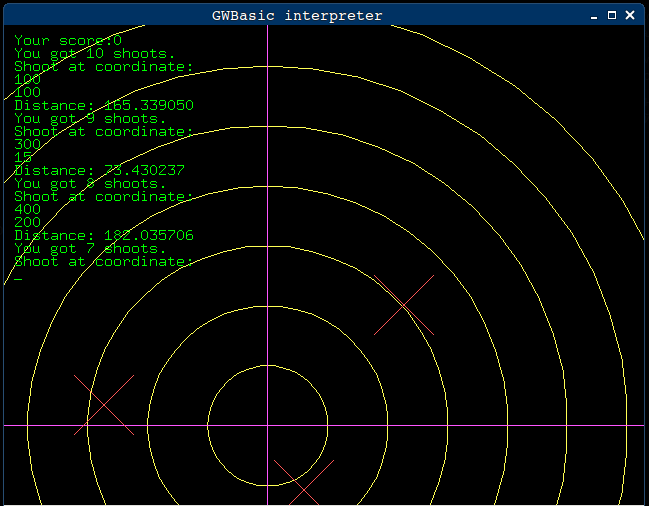
\includegraphics[scale=0.6]{gwbasic_screenshot.jpg}}
			\caption{Консоль графического режима в процессе игры.}
			\label{fig:testGame}
		\end{figure}
	\clearpage
	\part*{\centering Заключение}
	\hspace{\parindent}В данной работе была рассмотрена реализации среды GW-Basic c использованием средств {\it flex, bison, OpenGL, glut} на языке {\it C}. Возможности среды можно лекго расширить путем редактирования грамматики, а также добавлением обработчиков для соответствующих вершин дерева синтаксического разбора. 
	\addcontentsline{toc}{part}{Заключение}
	\newpage
	\nocite{*}
	\bibliographystyle{plain}		
	\bibliography{biblio}	
	\newpage

	\tableofcontents %Содержание
	\newpage 

	\part*{Приложение A. Тестовая программа на GW-Basic}
	%\addcontentsline{toc}{part}{Приложение A. Тестовая программа на GW-Basic}
	\lstinputlisting[basicstyle=\footnotesize]{circles.bas}
	% приложение
\end{document}
